\documentclass{article}
\usepackage[utf8]{inputenc}
\usepackage[margin=1in]{geometry}
\usepackage{amsmath, amsfonts}
\usepackage{fancyhdr}
\usepackage{multicol}
\usepackage{graphicx}
\graphicspath{ {images/} }
\pagestyle{empty}
\fancyhf{}
\cfoot{\thepage}

\lhead{MATB42: Assignment \#1 \\
Bonus}
\rhead{
Poon, Keegan\\
1002423727\\
Jan 23rd 2018}

\renewcommand{\headrulewidth}{0pt}
\begin{document}

\thispagestyle{fancy}

\begin{enumerate}
    \item Show that $\displaystyle \int_{-\pi}^{\pi} \sin (kx) \sin (nx) dx = 
    \begin{cases}
    0 &,\ k \not = \pm n \\
    \pm \pi &,\ k = \pm n \not = 0
    \end{cases}$
    
    Assuming $k \not = \pm n$
    \begin{align*}
    & \int_{-\pi}^{\pi} \sin (kx) \sin (nx) dx \\ &= \frac{1}{2}\int_{-\pi}^{\pi} \cos (kx - nx) - \cos (kx + nx) dx & \big[ \sin(A)\sin(B) = \frac{1}{2}[\cos(A-B) - \cos(A+B)]\big]\\ 
    &= \frac{1}{2}\Bigg[\int_{-\pi}^{\pi} \cos ((k - n)x)dx -\int_{-\pi}^{\pi} \cos ((k + n)x) dx \Bigg]\\
    &= \frac{1}{2}\Bigg[ \frac{1}{k-n}\Big[sin(kx)\Big]^\pi_{-\pi} - \frac{1}{k-n}\Big[sin(kx)\Big]^\pi_{-\pi} \Bigg] & \big[\text{Since cos is even}\big] \\
    & k,n \in \mathbb{Z} \implies (k \pm n) \in \mathbb{Z}, \ \text{but } \forall z \in \mathbb{Z}, \ \sin(z\pi) = 0 \\
    &= 0
    \end{align*}
    
    Assuming $k  = \pm n$
    \begin{align*}
    & \int_{-\pi}^{\pi} \sin (kx) \sin (nx) dx \\
    &= \int_{-\pi}^{\pi} \sin (kx) \sin (\pm kx) dx \\
    &= \pm \int_{-\pi}^{\pi} \sin^2 (kx) dx & \big[\text{Since sin odd}\big]\\
    &= \pm \int_{-\pi}^{\pi} \frac{1 - \cos(2kx)}{2} dx\\
    &= \pm\frac{1}{2} \Bigg[\int_{-\pi}^{\pi}1 dx - \int_{-\pi}^{\pi} \cos(2kx)dx \Bigg] \\
    &= \pm\frac{1}{2} \Bigg[2\pi - 0\Bigg] & \big[\text{Since cos even}\big] \\
    &= \pm \pi
    \end{align*}
    \newpage

    \item For each of the following functions, find the $N^{\text{th}}$ Fourier polynomial, assuming them to be periodic with period $2\pi$. Use symbolic algebra software to graph the first three approximations together with the original function.
    \begin{enumerate}
        \item $f(x) = x^2 , \ -\pi < x \leq \pi$
        \begin{multicols}{2}
        \begin{align*}
            a_0 &= \frac{1}{\pi}\int_{-\pi}^\pi x^2 dx \\
            &= \frac{2}{3\pi} \Big[x^3\Big]^\pi_0 &[\text{Since $x^2$ is even}]\\
            &= \frac{2\pi^2}{3} \\
        \end{align*}
        \begin{align*}
        \\
            b_k &= \frac{1}{\pi}\int_{-\pi}^\pi x^2\sin(kx) dx \\
            &= 0 &[\text{Since $x^2$ is even but sin is odd}]\\ 
        \end{align*}
        \end{multicols}
        \begin{align*}
            a_k &= \frac{1}{\pi}\int_{-\pi}^\pi x^2\cos(kx) dx \\
            &= \frac{2}{\pi}\int_{0}^\pi x^2\cos(kx) dx &[\text{Since $x^2$ and cos are even}]\\ 
			&\text{Let $u = x^2, du = 2xdx, dv = \cos(kx) dx, v = \frac{\sin(kx)}{k}$} \\
            &= \frac{2}{\pi}\Bigg[\Big[\frac{1}{k}x^2\sin(kx)\Big]^{\pi}_{0} - \frac{2}{k}\int_{0}^\pi x\sin(kx) dx \Bigg] \\
			&\text{Let $u = x, du = 1 dx, dv = \sin(kx) dx, v = -\frac{\cos(kx)}{k}$} \\
            &= \frac{2}{\pi}\Bigg[\Big[\frac{1}{k}x^2\sin(kx)\Big]^{\pi}_{0} - \frac{2}{k} \Big( \Big[ -\frac{1}{k}x\cos(kx)\Big]^\pi_0 - \frac{1}{k} \int^\pi_0 -\cos(kx) dx \Big) \Bigg] \\
            &= \frac{2}{\pi}\Bigg[\Big[\frac{1}{k}x^2\sin(kx)\Big]^{\pi}_{0} - \frac{2}{k} \Big( \Big[ -\frac{1}{k}x\cos(kx)\Big]^\pi_0 + \frac{1}{k^2} \Big[\sin(kx)\Big]^\pi_0 \Big) \Bigg] \\
            &= \frac{2}{\pi}\Bigg[0 - \frac{2}{k} \Big( \Big[ -\frac{1}{k}x\cos(kx)\Big]^\pi_0 + 0 \Big) \Bigg] \\
			&=-\frac{4}{k\pi} \Big[ -\frac{1}{k}x\cos(kx)\Big]^\pi_0 \\
			&= \frac{4}{k^2}\cos(k\pi) - 0  \\
			&= \frac{4}{k^2}(-1)^k
        \end{align*}
        Therefore the $N^{th}$ Fourier polynomial is 
        \[
        F_N(x) = \frac{\pi^2}{3} + \sum^N_{k=1} \frac{4}{k^2}(-1)^k\cos(kx)
        \]
        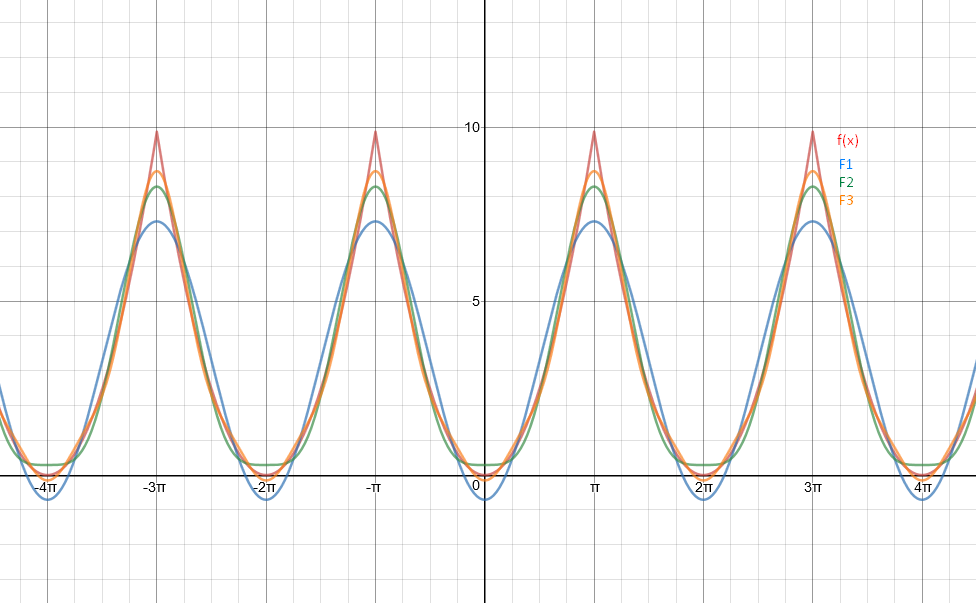
\includegraphics[width=\textwidth, angle=90]{b422a}
        \item $\displaystyle f(x) = \begin{cases}
                                        0 &, -\pi \leq x < 0 \\
                                        x &,  0 \leq x < \pi \\
                                    \end{cases}$
        \begin{align*}
            a_0 &= \frac{1}{\pi} \int_{-\pi}^{\pi}f(x) dx \\
            &= \frac{1}{\pi} \Bigg[\int_{-\pi}^{0}f(x) dx + \int_{0}^{\pi}f(x) dx \Bigg] \\
            &= \frac{1}{\pi} \Bigg[ 0 + \int_{0}^{\pi}x dx \Bigg] \\
            &= \frac{1}{\pi} \Bigg[\frac{1}{2}\Big[x^2\Big]_{0}^{\pi} \Bigg] \\
            &= \frac{\pi}{2}
        \end{align*}
        \begin{multicols}{2}
        \begin{align*}
            a_k &= \frac{1}{\pi} \int_{-\pi}^{\pi}f(x)\cos(kx) dx \\
            &= \frac{1}{\pi} \Bigg[\int_{-\pi}^{0}0 dx + \int_{0}^{\pi}x\cos(kx) dx\Bigg] \\
            &\text{Let } u = x,\: du = dx,\: dv = \cos(kx),\: v = \frac{1}{k}\sin(kx) \\
            &= \frac{1}{\pi} \Bigg[\frac{1}{k}\Big[x\sin(kx)\Big]^{\pi}_{0} - \frac{1}{k}\int_{0}^{\pi}\sin(kx) dx\Bigg] \\
            &= - \frac{1}{k\pi} \Bigg[\int_{0}^{\pi}\sin(kx) dx\Bigg] \\
            &= \frac{1}{k^2\pi} \Big[\cos(kx) \Big]_{0}^{\pi}\\
            &= \frac{(-1)^{-k} - 1}{k^2\pi} \\
        \end{align*}
        \begin{align*}
            b_k &= \frac{1}{\pi} \int_{-\pi}^{\pi}f(x)\sin(kx) dx \\
            &= \frac{1}{\pi} \Bigg[\int_{-\pi}^{0}0 dx +  \int_{0}^{\pi}x\sin(kx) dx \Bigg]\\
            &\text{Let } u = x,\: du = dx,\: dv = \sin(kx),\: v = -\frac{1}{k}\cos(kx) \\
            &= \frac{1}{\pi} \Bigg[-\frac{1}{k}\Big[x\cos(kx)\Big]^{\pi}_{0} + \frac{1}{k}\int_{0}^{\pi}\cos(kx) dx \Bigg]\\
            &= \frac{1}{k \pi} \Bigg[-\pi\cos(k\pi) + \frac{1}{k} \Big[ \sin(kx) \Big]_{0}^{\pi} \Bigg]\\
            &= \frac{1}{k \pi} \Bigg[-\pi\cos(k\pi) + 0 \Bigg]\\
            &= \frac{(-1)^{k+1}}{k}
        \end{align*}
        \end{multicols}
        Therefore the $N^{th}$ Fourier polynomial is 
        \[
        F_N(x) = \frac{\pi}{4} + \sum^N_{k=1}\Bigg[ \frac{(-1)^k-1}{k^2\pi}\cos(kx) + \frac{(-1)^{k+1}}{k} \sin(kx) \Bigg]
        \]
        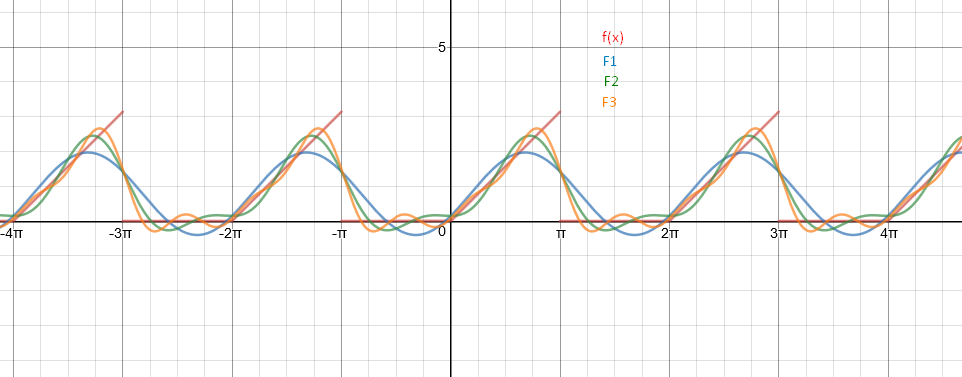
\includegraphics[width=\textwidth, angle=90]{b422b}
    \end{enumerate}
    \newpage
    \item Find the Fourier series for the function f(x) having period $2\pi$, one period of which is given by
        \[
        \displaystyle f(x) = \begin{cases}
                                    1 &,  0 \leq x < \pi \\
                                    x &,  \pi \leq x < 2\pi \\
                                \end{cases}
        \]
        \begin{multicols}{2}
        \begin{align*}
            a_0 &= \frac{1}{\pi} \int^{\pi}_{-\pi}f(x)dx\\
            &= \frac{1}{\pi} \Bigg[ \int^\pi_{0}f(x)dx + \int^{0}_{-\pi}f(x)dx \Bigg] \\
            &= \frac{1}{\pi} \Bigg[ \int^\pi_{0}1dx + \int^{2\pi}_{\pi}xdx \Bigg] &[\text{Period 2$\pi$}]\\
            &= \frac{1}{\pi} \Bigg[ \pi + \Big[ \frac{x^2}{2} \Big]^{2\pi}_{\pi} \Bigg] \\
            &= \frac{1}{\pi} \Bigg[ \pi +  \frac{4\pi^2}{2} - \frac{\pi^2}{2} \Bigg] \\
            &= 1 +  \frac{3\pi}{2}  \\
        \end{align*}
        \begin{align*}
            a_k &= \frac{1}{\pi} \int_{-\pi}^{\pi}f(x)\cos(kx)dx\\
            &= \frac{1}{\pi}\Bigg[ \int_{0}^{\pi}\cos(kx)dx+\int_{\pi}^{2\pi}x\cos(kx)dx \Bigg] \:[\text{Period 2$\pi$}]\\
            &\text{Let } u = x,\: du = dx,\: dv = \cos(kx),\: v = \frac{1}{k}\sin(kx) \\
            &= \frac{1}{\pi}\Bigg[ \frac{1}{k} \Big[\sin(kx)dx\Big]_{0}^{\pi}+\frac{1}{k}\Big[x\sin(kx) \Big]_{\pi}^{2\pi} - \frac{1}{k}\int_{\pi}^{2\pi} \sin(kx)dx\Bigg]\\
            &= \frac{-1}{k\pi}\Bigg[\int_{\pi}^{2\pi} \sin(kx)dx\Bigg]\\
            &= \frac{1}{k^2\pi}\Big[\cos(kx)dx\Big]_{\pi}^{2\pi}\\
            &= \frac{1 - (-1)^k}{k^2\pi}\\
        \end{align*}
        \end{multicols}
        \begin{align*}
            b_k &= \frac{1}{\pi} \int_{-\pi}^{\pi}f(x)\sin(kx) dx \\
            &= \frac{1}{\pi} \Bigg[\int_{0}^{\pi}\sin(kx)dx + \int_{\pi}^{2\pi}x\sin(kx)dx \Bigg]\:\:\:[\text{Period 2$\pi$}]\\
            &\text{Let } u = x,\: du = dx,\: dv = \sin(kx),\: v = -\frac{1}{k}\cos(kx) \\
            &= \frac{1}{\pi} \Bigg[\frac{-1}{k}\Big[\cos(kx)\Big]_{0}^{\pi} + \frac{-1}{k}\Big[x\cos(kx) \Big]_{\pi}^{2\pi} + \frac{1}{k}\int_{\pi}^{2\pi}\cos(kx)dx\Bigg]\\ 
            &= \frac{1}{k\pi} \Bigg[-\cos(k\pi) + 1 + -2\pi + \pi\cos(k\pi) + \int_{\pi}^{2\pi}\cos(kx)dx\Bigg]\\ 
            &= \frac{1}{k\pi} \Bigg[(\pi-1)(-1)^k+ 1 - 2\pi + \Big[\sin(kx)\Big]_{\pi}^{2\pi}\Bigg]\\ 
            &= \frac{1}{k\pi} \Bigg[(\pi-1)(-1)^k+ 1 - 2\pi\Bigg]\\ 
            &= \frac{(\pi-1)(-1)^k+ 1 - 2\pi}{k\pi} \\ 
        \end{align*}
        Therefore the Fourier series for $f(x)$ is 
        \[
        F(x) = \frac{2 + 3\pi}{4} + \sum_{k=1}^{\infty} \Bigg[\frac{1 - (-1)^k}{k^2\pi}\cos(kx) + \frac{(\pi-1)(-1)^k+ 1 - 2\pi}{k\pi}\sin(kx)\Bigg]
        \]
    \newpage
    \item Let $\displaystyle f(x) = \begin{cases}
                                        0 &, -\pi \leq x < -1 \\
                                        \frac{1}{2} &, -1 \leq x < 1 \\
                                        0 &, 1 \leq x < \pi
                                    \end{cases}$
    \begin{enumerate}
    \item What fraction of the energy of $f$ is contained in the constant term of its Fourier series?
    \begin{multicols}{2}
        \begin{align*}
            a_0 &= \frac{1}{\pi} \int^{\pi}_{-\pi}f(x)dx\\
            &= \frac{1}{\pi}\Bigg[ 0  + \int_{-1}^{1}\frac{1}{2}dx + 0 \Bigg]\\
            &= \frac{1}{\pi} \\
        \end{align*}
        \begin{align*}
            E(a_0) &= \frac{1}{2}a_0^2 \\
            &= \frac{1}{\pi}\Bigg[ 0  + \int_{-1}^{1}\frac{1}{4}dx + 0 \Bigg]\\
            &= \frac{1}{2\pi^2} \\
        \end{align*}
        \begin{align*}
            E(f) &= \frac{1}{\pi} \int^{\pi}_{-\pi}f(x)^2dx\\
            &= \frac{1}{\pi}\Bigg[ 0  + \int_{-1}^{1}\frac{1}{4}dx + 0 \Bigg]\\
            &= \frac{1}{2\pi} \\
        \end{align*}
        \begin{align*}
            \frac{E(a_0)}{E(f)} &= \frac{\frac{1}{2\pi^2}}{\frac{1}{2\pi}} \\
            &= \frac{1}{\pi} \\
            &\approx 32\%
        \end{align*}
    \end{multicols}
    \item Find a formula for the energy of the $k^{th}$ harmonic of $f$.
    \begin{multicols}{2}
    \begin{align*}
            a_k &= \frac{1}{\pi} \int_{-\pi}^{\pi}f(x)\cos(kx)dx\\
            &= \frac{1}{2\pi} \int_{-1}^{1}\cos(kx)dx\\
            &= \frac{1}{\pi} \int_{0}^{1}\cos(kx)dx &[\text{cos is even}] \\
            &= \frac{1}{k\pi} \sin(k) \\
            \end{align*}
    \begin{align*}
            b_k &= \frac{1}{\pi} \int_{-\pi}^{\pi}f(x)\sin(kx) dx \\
            &= 0 \; [\text{Since sin is odd and $f$ is even}] \\
    \end{align*}
    \begin{align*}
        E(k^{th} \text{ harmonic}) &= A_k^2 = \sqrt{a_k^2+b_k^2}^2 = a_k^2 \\
        &= \frac{\sin^2(k)}{k^2\pi^2}
    \end{align*}
    \end{multicols}
    \item How many terms of the Fourier series of $f$ are needed to capture 80\% of the energy of $f$?
    \begin{align*}
       \frac{\sin^2(k)}{k^2\pi^2}/\frac{1}{2\pi} = \frac{2\sin^2(1)}{1^2\pi} &\approx 45\%  \\
       \frac{2\sin^2(2)}{2^2\pi} &\approx 13\% \\
       32\% + 45\% + 13\% = 90\% &\geq 80\%
    \end{align*}
    Including the constant term, three terms are required to capture $80\%$ of the energy of $f$.
    \item Find $F_N$, the $N^{th}$ Fourier polynomial of $f$, and use symbolic algebra software to graph $f$ and $F_3$ on the interval $[-3\pi,3\pi]$.
    \[
    F_N(x) = \frac{1}{2\pi} + \sum^N_{k=1}\Bigg[ \frac{\sin(k)}{k\pi}\cos(kx) \Bigg]
    \]
    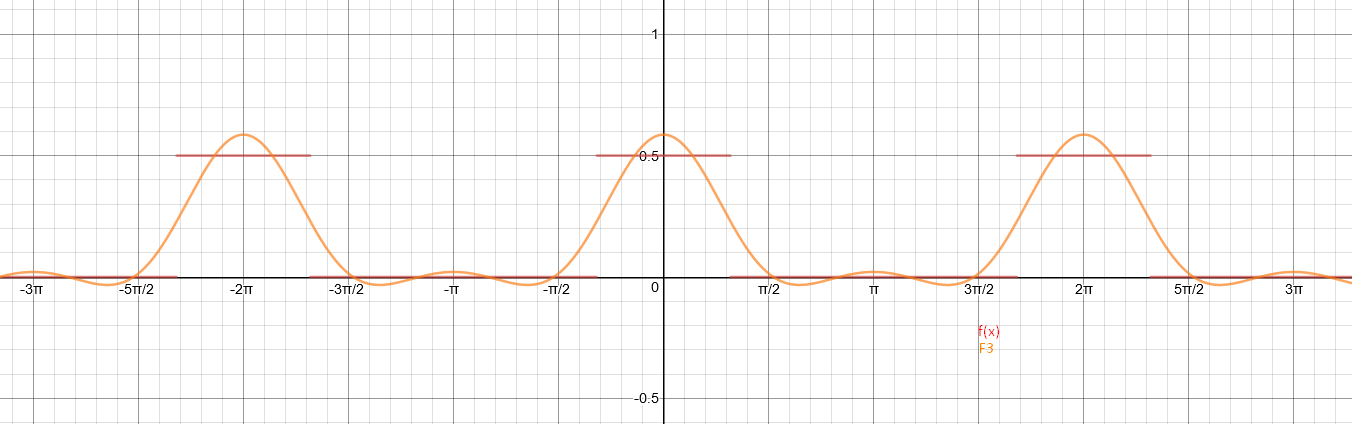
\includegraphics[width=\textwidth, angle=90]{b424d}
    \end{enumerate}
    \newpage
    \item Find the Fourier series for the function $f(x)$ (of period 4) which corresponds to $y=x^2-4$ on the interval $[-2,2]$.
    \begin{multicols}{2}
    \begin{align*}
            a_0 &= \frac{2}{4} \int^{2}_{-2}f(x)dx\\
            &= \int^{2}_{0}x^2-4dx \:\:\: [\text{$f(x)$ is even}]\\
            &= \Bigg[ \frac{1}{3}\Big[x^3\Big]_{0}^{2} - 4\Big[x\Big]_{0}^{2} \Bigg] \\
            &= \Bigg[ \frac{8}{3} - 8 \Bigg]\\
            &= -\frac{16}{3}
    \end{align*}
    \begin{align*}
            b_k &= \frac{1}{2} \int^{2}_{-2}f(x)\sin\Big(\frac{2\pi kx}{4}\Big)dx\\
            &= 0 \: [\text{Since $f$ is even, but sin is odd}]
    \end{align*}
    \begin{align*}
            a_k &= \frac{1}{2} \int^{2}_{-2}f(x)\cos\Big(\frac{2\pi kx}{4}\Big)dx\\
            &= \int^{2}_{0}(x^2-4)\cos\Big(\frac{\pi kx}{2}\Big)dx \:\:\: [\text{$f(x)$ and cos are even}]\\
            &= \int^{2}_{0}x^2\cos\Big(\frac{\pi kx}{2}\Big)dx - 4\int^{2}_{0}\cos\Big(\frac{\pi kx}{2}\Big)dx\\
			&\text{Let $u = x^2, du = 2xdx, dv = \cos\Big(\frac{\pi kx}{2}\Big) dx, v = \frac{2\sin(\frac{\pi kx}{2})}{k\pi}$} \\
            &= \frac{2}{k\pi}\Big[x^2 \sin\Big(\frac{\pi kx}{2}\Big)\Big]^{2}_{0} - \frac{4}{k\pi}\int^{2}_{0}x\sin\Big(\frac{\pi kx}{2}\Big)dx  \\
            & \:\:\: -\frac{8}{k \pi}\Big[\sin\Big(\frac{\pi kx}{2}\Big)\Big]^{2}_{0}\\
            &= \frac{8}{k \pi}\sin\Big(\frac{\pi kx}{2}\Big) - \frac{4}{k\pi}\int^{2}_{0}x\sin\Big(\frac{\pi kx}{2}\Big)dx - \frac{8}{k \pi}\sin\Big(\frac{\pi kx}{2}\Big)\\
			&\text{Let $u = x, du = 1 dx, dv = \sin\Big(\frac{\pi kx}{2}\Big) dx, v = -\frac{2\cos(\frac{\pi kx}{2})}{k\pi}$} \\
            &= - \frac{4}{k\pi}\Bigg[-\frac{2}{k\pi}\Big[x\cos\Big(\frac{\pi kx}{2}\Big)\Big]^{2}_{0} + \frac{2}{k\pi}\int^{2}_{0}\cos\Big(\frac{\pi kx}{2}\Big) dx\Bigg] \\
            &= - \frac{4}{k\pi}\Bigg[-\frac{4\cos(\pi k)}{k\pi} + \frac{2}{k^2\pi^2}\Big[\sin\Big(\frac{\pi kx}{2}\Big) \Big]^{2}_{0} \Bigg]\\
            &= - \frac{4}{k\pi}\Bigg[-\frac{4(-1)^k}{k\pi} + \frac{\sin(\pi k)}{k^2\pi^2} \Bigg]\\
            &=  \frac{16(-1)^k}{k^2\pi^2}
    \end{align*}
    \end{multicols}
    
    Therefore the Fourier series for $f(x)$ is 
        \[
        F(x) = - \frac{8}{3} + \sum_{k=1}^{\infty} \frac{16(-1)^k}{k^2\pi^2}\cos(kx)
        \]
    \newpage
    \item
    \begin{enumerate}
        \item Suppeose $f(x)$ has a continuous derivative $f'(x)$ on $[0,2\pi]$. Let $a_k$ and $b_k$ the $k^{th}$ Fourier coefficients of $f$ and let $a'_k$ and $b'_k$ be those of $f'$. Show that
        \begin{align*}
            a'_k \: &= \: kb_k + \frac{f(2\pi)-f(0)}{\pi} \\
            b'_k \: &= \: -ka_k.
        \end{align*}
        \begin{align*}
            &\text{By definition, } \\
            a'_k &= \frac{1}{\pi}\int_{0}^{2\pi}f'(x)\cos(kx)dx\\
            \text{Let }&u = \cos(kx), du = -k\sin(kx)dx, dv = f'(x)dx , v = f(x) \\
            &= \frac{1}{\pi}\Bigg[\Big[f(x)\cos(kx)\Big]^{2\pi}_{0} + k\int_{0}^{2\pi}\sin(kx)f(x)dx\Bigg] \\
            &= \frac{1}{\pi} \Bigg[ \Big[ f(x)\cos(kx) \Big]^{2\pi}_{0}  + k\pi \Big[\frac{1}{\pi}\int_{0}^{2\pi}\sin(kx)f(x)dx\Big]\Bigg] \\            
            &= \frac{1}{\pi} \Bigg[ f(2\pi)\cos(2k\pi) - f(0)\cos(0) + k\pi b_k\Bigg] \: [\text{Def of $b_k$}] \\
            &= \frac{1}{\pi} \Bigg[ f(2\pi) - f(0) + k\pi b_k\Bigg] \\
            &= kb_k + \frac{f(2\pi) - f(0)}{\pi} \: \text{As wanted}
        \end{align*}
        \begin{align*}
            &\text{By definition, } \\
            b'_k &= \frac{1}{\pi}\int_{0}^{2\pi}f'(x)\sin(kx)dx\\
            \text{Let }&u = \sin(kx), du = k\cos(kx)dx, dv = f'(x)dx , v = f(x) \\
            &= \frac{1}{\pi}\Bigg[\Big[f(x)\sin(kx)\Big]^{2\pi}_{0} - k\int_{0}^{2\pi}\cos(kx)f(x)dx\Bigg] \\
            &= \frac{1}{\pi} \Bigg[ \Big[ f(x)\sin(kx) \Big]^{2\pi}_{0}  - k\pi \Big[\frac{1}{\pi}\int_{0}^{2\pi}\cos(kx)f(x)dx\Big]\Bigg] \\            
            &= \frac{1}{\pi} \Bigg[ -f(2\pi)\sin(2k\pi) + f(0)\sin(0) - k\pi a_k\Bigg] \: [\text{Def of $a_k$}] \\
            &= -ka_k \: \text{As wanted}
        \end{align*}
        \newpage
        \item Use part (a) to find all the Fourier coefficients of the restriction of $f(x) = e^{\lambda x}$ to the interval $[0,2\pi]$ in terms of the constant $\lambda$.
        \paragraph{}
        Since $\frac{d}{dx}e^{\lambda x} = \lambda e^{\lambda x}$, the coefficients of every term of the Fourier polynomial of the derivative function will simply be that of the original, multiplied by $\lambda$.
        \begin{multicols}{2}
        \noindent
        \begin{align*}
        \lambda a_k &= kb_k + \frac{e^{2\pi\lambda} - 1}{\pi} \\
        \lambda a_k &= -k\Big(\frac{ka_k}{\lambda}\Big) + \frac{e^{2\pi\lambda} - 1}{\pi} \\
        \lambda a_k + \frac{k^2a_k}{\lambda}&= \frac{e^{2\pi\lambda} - 1}{\pi} \\
        a_k \Big(\lambda  + \frac{k^2}{\lambda}\Big)&= \frac{e^{2\pi\lambda} - 1}{\pi} \\
        a_k &= \frac{e^{2\pi\lambda} - 1}{\pi(\lambda  + \frac{k^2}{\lambda})} \\
        a_k &= \frac{e^{2\pi\lambda} - 1}{\frac{\pi(\lambda^2 + k^2)}{\lambda}} \\
        a_k &= \frac{\lambda(e^{2\pi\lambda} - 1)}{\pi(\lambda^2 + k^2)} \\
        \end{align*}
        \begin{align*}
        \lambda b_k &= -ka_k \\
        b_k &= -\frac{ka_k}{\lambda} \\
        b_k &= -\frac{k}{\lambda}\Big(\frac{\lambda(e^{2\pi\lambda} - 1)}{\pi(\lambda^2 + k^2)}\Big) \\
        b_k &= -\frac{k(e^{2\pi\lambda} - 1)}{\pi(\lambda^2 + k^2)}
        \end{align*}
        \end{multicols}
    \end{enumerate}
    \newpage
        
    \item Find two Fourier expansions for the restriction of the function $f(x) = \sin x$ to the interval $[0,\pi]$. In one expansion all the sine terms should have zero coefficient, in the other all cosine terms should have coefficient.
    
    Even expansion (sine terms have zero coefficient)
    \begin{align*}
        f(-x) &= 
        \begin{cases}
            -\sin(x),&\text{if } -\pi \leq x < 0\\
            \sin(x), &\text{if } 0 \leq x < \pi
        \end{cases} \\&\text{This works since sin odd, so $-\sin(-x) = \sin(x)$} 
    \end{align*}
    \begin{multicols}{2}    
    \noindent
    \begin{align*}
        a_k &= \frac{1}{\pi}\int_{-\pi}^{\pi}f(x)\cos(kx)dx \\ 
        &= \frac{2}{\pi} \int_{0}^{\pi}\sin(x)\cos(kx)dx \\
        &= \frac{1}{\pi} \Bigg[ \int_{0}^{\pi}\sin((k+1)x)dx - \int_{0}^{\pi}\sin((k-1)x)dx\Bigg]\\
        &= \frac{1}{\pi} \Bigg[- \frac{1}{k+1}\Big[\cos((k+1)x) \Big]_{0}^{\pi} + \frac{1}{k-1}\Big[\cos((k-1)x)\Big]_{0}^{\pi}\Bigg]\\
        &= \frac{1}{\pi} \Bigg[- \frac{(-1)^{(k+1)} -1}{k+1} + \frac{(-1)^{(k-1)} -1}{k-1}\Bigg]\\
        &= \frac{(-1)^{(k+1)} -1}{\pi} \Bigg[\frac{1}{k-1} - \frac{1}{k+1}\Bigg]\\
        &= \frac{(-1)^{(k+1)} -1}{\pi} \Bigg[\frac{k + 1 - k + 1}{k^2-1^2}\Bigg]\\
        &= 2\frac{(-1)^{(k+1)} -1}{\pi(k^2 - 1)} [\text{Valid for $ k > 1$}] \\
        &\text{For k = 1}\\
        &= \frac{1}{\pi} \Bigg[ \int_{0}^{\pi}\sin(2x)dx - \int_{0}^{\pi}\sin((1-1)x)dx\Bigg]\\
        &= \frac{1}{\pi} \int_{0}^{\pi}\sin(2x)dx \\
        &= -\frac{1}{2\pi}\Big[\cos(2x)\Big]_{0}^{\pi} \\
        &= -\frac{1}{2\pi}\Big[1 - 1\Big] \\
        &= 0 \\
    \end{align*}
    \begin{align*}
        a_0 &= \frac{1}{\pi}\int_{-\pi}^{\pi}f(x)dx \\ 
        &= \frac{2}{\pi}\int_{0}^{\pi}f(x)dx\: [\text{Defined to be even}] \\ 
        &= \frac{2}{\pi} \int_{0}^{\pi}\sin(x)dx \\ 
        &= \frac{2}{\pi}\Bigg[- \Big[\cos(x)\Big]_{0}^{\pi} \Bigg] \\ 
        &= \frac{2}{\pi} \Bigg[ 1 + 1 \Bigg] \\ 
        &= \frac{4}{\pi}
    \end{align*}
    \begin{align*}
        b_k &= 0 & [\text{Since $f$ defined even}]
    \end{align*}
        Therefore the even Fourier expansion for $f(x)$ is 
        \[
        F_N = \frac{2}{\pi} + \sum_{k=2}^{\infty} 2\frac{(-1)^{(k+1)} -1}{\pi(k^2 - 1)}
        \]

    \end{multicols}
    \newpage
    Odd expansion (cosine terms have zero coefficient)
    \begin{align*}
        f(-x) = \sin(x), \: \text{on }[-\pi, \pi]
    \end{align*}
    This works, since sin is already an odd function
    \begin{multicols}{2}
    \noindent
    \begin{align*}
        a_0 &= \frac{1}{\pi}\int_{-\pi}^{\pi}f(x)dx \\ 
        &= \frac{1}{\pi}\int_{-\pi}^{\pi}\sin(x)dx \\ 
        &= 0 \: [\text{sin is odd}]
    \end{align*}
    \begin{align*}
        a_k &= \frac{1}{\pi}\int_{-\pi}^{\pi}f(x)\cos(kx)dx \\ 
        &= \frac{1}{\pi}\int_{-\pi}^{\pi}\sin(x)\cos(kx)dx \\ 
        &= 0 \: [\text{sin is odd, cos even}]
    \end{align*}
    \begin{align*}
        b_k &= \frac{1}{\pi}\int_{-\pi}^{\pi}f(x)\sin(kx)dx \\ 
        &= \frac{1}{\pi}\int_{-\pi}^{\pi}\sin(x)\sin(kx)dx \\ 
        &= 1 \text{ if } k = 1, \text{ 0 otherwise [Refer to q1]}
    \end{align*}
    \end{multicols}
    So the Fourier expansion is simply $\sin(x)$
\end{enumerate}

    \newpage

\section*{Bonus}
Find the Fourier series for the function $y = f(x)$ of period $2\pi$ , if one period is given by
\[ f(x) =
    \begin{cases}
        -\frac{1}{2}-\frac{x}{2\pi} &, -\pi \leq x < 0 \\
        \frac{1}{2}-\frac{x}{2\pi} &, 0 \leq x < \pi
    \end{cases}
\]
This function is odd over the period since $(-\frac{1}{2}-\frac{-x}{2\pi} ) =(-\frac{1}{2}+\frac{x}{2\pi}) = - (\frac{1}{2} - \frac{x}{2\pi} )$ \\
\begin{multicols}{2}
    \noindent
    \begin{align*}
        a_0 &= \frac{1}{\pi}\int_{-\pi}^{\pi}f(x)dx \\ 
        &= 0 \: \: \: [\text{Since $f$ odd}] \\
        a_k &= \frac{1}{\pi}\int_{-\pi}^{\pi}f(x)\cos(kx)dx \\ 
        &= 0 \: \: \: [\text{Since $f$ odd and cos even}] \\
        \end{align*}
        \begin{align*}
        \text{ Therefore the Fourier series for $f(x)$ is} \\
        F(x) = \sum_{k=1}^{\infty}\frac{1}{k\pi}\sin(kx) 
    \end{align*}
    \begin{align*}
        b_k &= \frac{1}{\pi}\int_{-\pi}^{\pi}f(x)\sin(kx)dx \\ 
        &= \frac{1}{\pi} \Bigg[\int_{-\pi}^{0}\Big[-\frac{1}{2}-\frac{x}{2\pi}\Big]\sin(kx)dx + \int_{0}^{\pi}\Big[\frac{1}{2}-\frac{x}{2\pi}\Big]\sin(kx)dx \Bigg]\\ 
        &= \frac{1}{\pi} \Bigg[-\int_{-\pi}^{0}\Big[\frac{(\pi+x)\sin(kx)}{2\pi}\Big]dx + \int_{0}^{\pi}\Big[\frac{(\pi-x)\sin(kx)}{2\pi}\Big]dx \Bigg]\\ 
        &\text{Let $u = (\pi+x), du = 1 dx, dv = \sin(kx) dx, v = -\frac{\cos(kx)}{k}$} \\
        &= \frac{1}{2\pi^2} \Bigg[ \int_{0}^{\pi}\Big[(\pi-x)\sin(kx)\Big]dx + \Big[(\pi+x)\frac{\cos(kx)}{k}\Big]_{-\pi}^{0}\\ 
        & \: \: \: - \int_{-\pi}^{0}\frac{\cos(kx)}{k}dx \Bigg] \\
        &= \frac{1}{2\pi^2} \Bigg[ \int_{0}^{\pi}\Big[(\pi-x)\sin(kx)\Big]dx + \frac{\pi}{k} - \frac{1}{k^2}\Big[\sin(kx)\Big]_{-\pi}^{0} \Bigg] \\
        &= \frac{1}{2\pi^2} \Bigg[ \int_{0}^{\pi}\Big[(\pi-x)\sin(kx)\Big]dx + \frac{\pi}{k} \Bigg] \\
        &\text{Let $u = (\pi-x), du = -1 dx, dv = \sin(kx) dx, v = -\frac{\cos(kx)}{k}$} \\
        &= \frac{1}{2\pi^2} \Bigg[- \Big[\frac{(\pi - x)\cos(kx)}{k}\Big]_{0}^{\pi} - \int_{0}^{\pi}\frac{\cos(kx)}{k}dx + \frac{\pi}{k} \Bigg] \\
        &= \frac{1}{2\pi^2} \Bigg[ \frac{\pi}{k} - \Big[\frac{\sin(kx)}{k^2}\Big]_{0}^{\pi}+ \frac{\pi}{k} \Bigg] \\
        &= \frac{1}{k\pi}
        \end{align*}
\end{multicols}

\end{document}
